\clearpage
\section{Literature}
\subsection{Background:}
This section will look at how clouds and rain are generated currently in games.
Weather plays a huge impact to the how a game feels, as \citet{Barton08} wrote about how "It was a dark and stormy night" not only sets the time and weather of the scene but also sets the tone.
\citet{NWang04} agrees by saying that one of the most fascinating parts of a scene could be the clouds.
An example of this is the game Tomb Raider (\citeyear{TombRaider13}) which at numerous points in the game the user can see a vast sky full of clouds as seen in Figure \ref{fig:tomb_raider}. 

\begin{figure}[ht!]
	\centering
	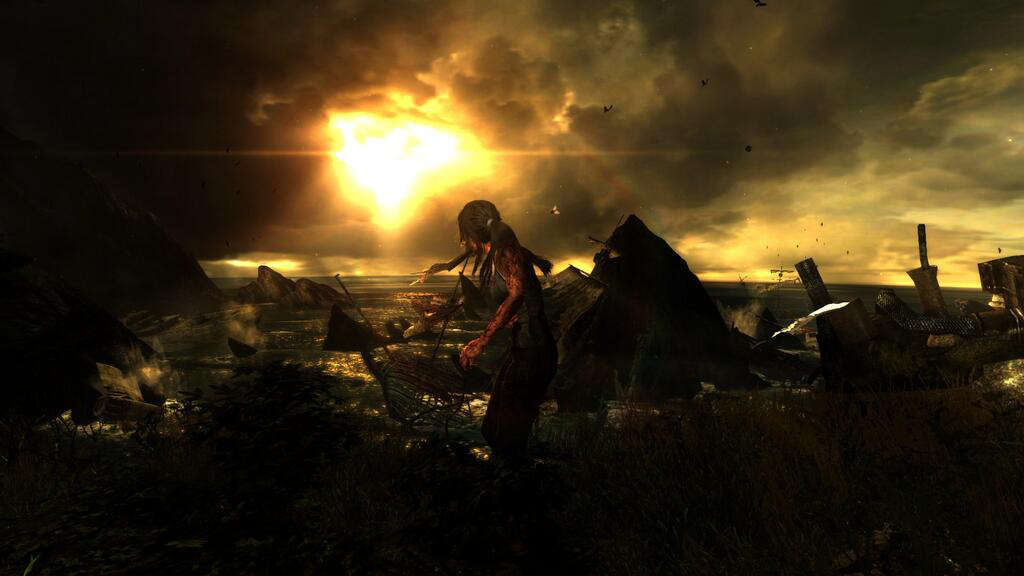
\includegraphics[width=\textwidth]{images/tomb_raider.PNG}
	\caption{A screenshot from Tomb Raider (\citeyear{TombRaider13})}
	\label{fig:tomb_raider}
\end{figure}


\subsection{Cloud Generation:}
\label{sec:cg}
There are a number of different methods for generating clouds from cellular automaton, to fluid dynamic equations, to importing 3D objects.

\subsubsection{Artist Created:}
\label{sec:art}
This technique works not by creating the clouds at run time but instead creates the clouds as models and loads them into the game when needed.
\citet{NWang04} describes a version of this which allows artists to create boxes in 3DS Max in which a plug-in will then generate clouds inside the box.
She explained how this method was used when creating Microsoft Flight Simulator 2004: A Century of Flight (\citeyear{MFS03}).
A similar method can be used in the CryEngine 3 SDK (\citeyear{Crytek13}) which allows the user to alter the properties of the clouds created in real-time within the editor. 
This method can create very realistic looking clouds but doesn't allow for realistic movement or generation.
\subsubsection{Cellular Automata (CA):}
\label{sec:ca}
A Cellular Automaton can be described as a regular shaped structure which consists of identical cells that are computed synchronously depending on the state of the cell and its neighbours \citep{SDantchev11}.
\citet{DobashiEtAl00} used a cellular automaton model when generating the clouds which involved giving each cell a number of boolean states that, when coupled with the rules generated clouds.

This method was extended by \citet{Miyazaki01} who used the Coupled Map Lattice (CML) method which is described as “an extension of cellular automaton, and the simulation space is subdivided into lattices”.
\citet{Miyazaki01} also goes on to explain that the CML model differs from the CA model by using continuous values instead of discreet values.
This CML model uses very simple equations for viscosity and pressure effects, advection, diffusion of water vapour, thermal diffusion and buoyancy, and the transition from vapour to water.

Cellular Automaton gives a lot more control to the physics of clouds because of the equations used to define them compared to clouds created by artists.
However these equations are not as accurate as using fluid dynamic equations to move and generate clouds.
\subsubsection{Fluid Dynamics:}
\label{sec:fd}
As clouds can be described as an incompressible fluid it can be simulated via the fluid dynamic equations.
The Navier-Stokes Equations are used for a “fluid that conserves both mass and momentum.” \citep{JStam99}.
In the Navier-Stokes equation $\rho$ is the density, $\mathbf{f}$ represents all external forces and $\nu$ is the kinematic viscosity of the fluid.
The velocity and pressure are defined as $\mathbf{u}$ and $p$ respectively.
The second equation is the continuity equation which means the fluid is incompressible.
\begin{equation} \label{eq:Navier-Stokes}
  \centering
  \frac{\partial \mathbf{u}}{\partial t}=-\left(\mathbf{u}\cdot \nabla \right)\mathbf{u}-\frac{\nabla p}{\rho}+\nu{\nabla }^{2}\mathbf{u}+\mathbf{f}
\end{equation}
\begin{equation} \label{eq:Continuity Equation}
  \centering
  \nabla\cdot\mathbf{u}=0
\end{equation}
The Navier-Stokes equations (2.1) and (2.2) can be simplified to Euler's Equation because “the effects of viscosity are negligible in gases” \citep*{Fedkiw01}.
This makes the equations for generating the clouds less computationally heavy and can be shown in equation (2.3) which has no $\nu{\nabla }^{2}\mathbf{u}$.
The continuity equation has not changed and can be seen from (2.4) being the same as (2.2).
\begin{equation} \label{eq:Euler's Equation}
  \centering
   \frac{\partial \mathbf{u}}{\partial t}=-\left(\mathbf{u}\cdot \nabla \right)\mathbf{u}-\frac{\nabla p}{\rho}+\mathbf{f}
\end{equation}
\begin{equation} \label{eq:Continuity Equation Euler}
  \centering
  \nabla\cdot\mathbf{u}=0
\end{equation}
\citet*{Fedkiw01}, \citet{HarrisEtAl03}, and \citet*{DOverby02} all used work created by \citet{JStam99} on stable fluid simulations.
\citet*{DOverby02} used the actual solver created by \citet{JStam99} in the application to solve the fluid dynamic part of creating clouds.
Whereas \citet*{Fedkiw01} and \citet{HarrisEtAl03} used the theory in the creation of the smoke and clouds respectively.
Even though all three used the same start for simulating cloud generation they have different methods for assigning values to the other equations needed. 

The \citet*{Fedkiw01} model uses a Poisson equation to compute the pressure of the system and two scalar functions for advecting the temperature and density.
This model also uses a function built up of the temperature, ambient temperature, density, and two other positive constants to create a buoyancy effect.
The model also simulates velocity fields, which are dampened out on the coarse grid, by finding where the feature should be and then creating a realistic turbulent effect.

\citet*{DOverby02} computes the local temperature based upon the heat energy and the pressure.
The pressure is calculated from ground level to the tropopause by an exponentially decreasing value \citep*{DOverby02}.
The buoyancy in this model is created using the local temperature, the surrounding temperature and a buoyancy scalar.
Relative humidity is calculated based upon current water vapour and saturated water vapour.
Water condensation is then calculated based upon relative humidity, hygroscopic nuclei, and a condensation constants.
The final equation to be calculated is the latent heat which is calculated by the water condensation and a constant.
 
The \citet{HarrisEtAl03} model uses equations for water continuity, thermodynamics, buoyancy, and a Poisson equation for fluid flow.
This model also creates velocity fields using the same process as \citet*{Fedkiw01}.
This model uses more complicated equations than the previous two models to more accurately simulate the creation of clouds.
For example this model uses gravity, the mass mixing ratio of hydrometeors and virtual potential temperatures, whereas the previous models use scalars or other constants with the temperature to create the buoyancy force.

The vorticity confinement as defined by \citet{HarrisEtAl03} model is defined in equation \ref{eq:vc}.
$\omega$ is the vorticity, defined by $\omega = \nabla\times\mathbf{u}$, and $N$ is the normalized vorticty vector field and points from areas of lower vorticiy to areas of higher vorticity which is defined by equation \ref{eq:vcn}.
With $h$ is the grid scale and $\epsilon$ is I scale parameter.

\begin{equation} \label{eq:vc}
  \centering
  f_{vc} = \epsilon h\left(N\times\omega\right)
\end{equation}
\begin{equation} \label{eq:vcn}
  \centering
  N = \frac{\nabla\left|w\right|}{\left|\nabla\left|w\right|\right|}
\end{equation}

The buoyant force is defined in equation \ref{eq:bf} where $g$ is the acceleration due to gravity.
$q_{v}$ is the mixing ratio of hydrometeors and in this case is defined as $q_{c}$ the mixing ratio of liquid water.
$\theta_{v}$ is the virtual potential temperature and is defined in equation $\theta_{v} \approx \theta(1+0.61 q_{v})$.
$\theta_{v0}$ is the reference potential temperature and is between 290 and 300K as defined by \citet{HarrisEtAl03}.

\begin{equation} \label{eq:bf}
  \centering
  B = g\left(\frac{\theta_{v}}{\theta_{v0}} - q_{h}\right)
\end{equation}

The water continuity in \citet{HarrisEtAl03} model is based upon the Bulk Water Continuity model which described by \citet{houze1994cloud} as “the simplest type of cloud is a warm non-precipitating cloud”.
\citet{houze1994cloud} describes this model as using two categories to describe creating the cloud, these categories being vapour $q_{v}$ and cloud liquid water $q_{c}$.
This model is described as equations \ref{eq:wc} by \citet{houze1994cloud}.
$C$ is the condensation rate.

\begin{equation} \label{eq:wc}
  \centering
  \frac{Dq_{v}}{Dt} = - C,	\frac{Dq_{c}}{Dt} = C
\end{equation}

Thermodynamic Equation defined in \citet{HarrisEtAl03} model can be seen in equation \ref{eq:thermo}. $c_{p}$ is the specific heat capacities of dry air at constant pressure in this case $1005J kg^{-1} K^{-1}$. $L$ is the latent heat of vaporization of water which is $2.501 J kg^{-1}$.
The part of the equation in brackets on the right hand side of the equation can be exchanged for the condensation rate from the water continuity equations.

\begin{equation} \label{eq:thermo}
  \centering
  \frac{\partial\theta}{\partial t} + \left(\mathbf{u}\cdot\nabla\right)\theta = \frac{-L}{c_{p}\Pi}\left(\frac{\partial q_{v}}{\partial t} + \left(\mathbf{u\cdot\nabla}q_{v}\right)\right)
\end{equation}

$\Pi$ is called the Exner function and is defined in equation \ref{eq:exner}.
Where $p_{0}$ is the pressure at the surface, usually taken as $1000 hPa$; $R_{d}$ is the gas constant for dry air a can be taken as $287 J kg^{-1} K^{-1}$; $c_{p}$ is the heat capacity of dry air at constant pressure, and $p$ is pressure.

\begin{equation} \label{eq:exner}
  \centering
  \Pi = \left(\frac{p}{p_{0}}\right)^{\frac{R_{d}}{c_{p}}}
\end{equation}

With these extra equations using fluid dynamics for generating and moving clouds will give more accurate simulations compared to the previously mentioned processes. There is a draw back for using fluid dynamic equations as it will use more computing power compared to artists created, and Cellular Automaton methods. 
\subsection{Cloud Rendering:}
\label{sec:cr}
Due to the nature of clouds when light passes through them it becomes scattered.
The majority of the models looked at use two different techniques to accomplish this effect single scattering and multiple scattering.
These model may render clouds using these scattering techniques directly or may use scattering inside other rendering processes such as photon mapping.
A number of these models also use billboards or imposters when rendering the clouds as this saves on computation.
This section will look at single scattering, multiple scattering, and photon mapping. 
\subsubsection{Single Scattering:}
\citet*{MHarris01} describe single scattering as a model that simulates scattering in a single direction that is usually the direction leading to the point of view.
There are debates whether or not this type of rendering is detailed enough for rendering clouds.
\citet{Miyazaki01} states the main topic of his model is the cloud shapes so using single scattering is enough to check the shape of the cloud.
\citet{CBohren87} describes single scattering as insufficient when describing common observations. 
\subsubsection{Multiple scattering:}
\label{sec:multiple}
“Multiple scattering models are more physically accurate, but must account for scattering in all directions … and therefore are much more complicated and expensive to evaluate” \citep{MHarris01}.
\citet{HarrisEtAl03} uses a version of multiple scattering which is called multiple forward scattering, this differs from the original by instead of calculating scattering in all directions it calculates scattering in the forward direction only.
This means the algorithm is less computationally heavy. \citet*{Fedkiw01} describe the multiple scattering of light as necessary for objects made from water vapour, which clouds are.

\subsubsection{Photon Mapping:}
“Photon mapping is a variation of pure Monte Carlo ray tracing in which photons (particles of radiant energy) are traced through a scene” (\citet{Jensen96}, cited in \citet{MHarris03}).
\citet{MHarris03} describes the process of photon mapping as storing position, incoming direction, and radiance of each photon landing on a nonspecular surface that has been traced from the light source.
\citet*{Fedkiw01} use photon mapping when rendering smoke and describe the process as a two pass algorithm, one where a volume photon map is built and the second as a rendering pass using a forward ray marching algorithm.
\subsection{Rain Rendering:}
“Rain is an extremely complex natural atmospheric phenomenon” \citep*{APuig-Centelles09}.
\citet*{APuig-Centelles09} describe two main techniques for rendering rain to a scene scrolling textures where a texture the size of the screen scrolls in the direction of the rain, and a particle system where each rain drop is represented as a particle in the system.
\citet{STariq07} writes “animating rain using a particle system is more useful for realistic looking rain with lots of behaviour (like changing wind).”
Whereas \citet*{APuig-Centelles09} sates texture scrolling “is faster than particle systems, but it does not allow interaction between rain and the environment.”